\section{Exercise 1}
Decrypt the following ciphertext that was encrypted with a Caesar cipher:
\begin{center}
GJBFW JYMJN IJXTK RFWHM
\end{center}
To decrypt this we need to find the key used to shift the cipher relative to the
normal alphabet, as there are only 26 possibilities, this is easily
bruteforced.\\

\begin{lstlisting}
    for(int i = 0; i < 26; i++)
    {
    	for(int j = 0; j < cipherText.length; j++)
    	{
    		System.out.print(ciphertext[j] + i % 26);
    	}
    }
\end{lstlisting}

This gives us 26 examples of cleartext, the only one that resembles an english
cleartext is $p = c + 21 mod 26$:
\begin{center}
GJBFW JYMJN IJXTK RFWHM\\
BEWAR ETHEI DSOFM ARTCH\\
~\\
BEWARE THE IDES OF MARCH\\
\end{center}

\section{Exercise 3}
KPA was used under WW2 by the Bletchley park team, to break the engima codes, by 
used by the german forces. They found some plaintext by recognicing repeated
words like "Wetter" in daily weather-reports. CPA was also used against
enigma, here the Bletchley park team had the royal air force encourage
the german army to send messages about an alreaddy known area, for
example by seeding an area with mines, this would lead to messages
being send with names of ports or areas alreaddy known by the
analysts.\cite{SoN}\\

\section{Exercise 5}
Truthtable for XOR:
\begin{center}
	\begin{tabular}{ cc|c}
	  key & plain & output\\ \hline
	  0 & 0 & 0\\
	  0 & 1 & 1\\
	  1 & 0 & 1\\
	  1 & 1 & 0\\
	\end{tabular}
\end{center}
To implement this in code we take to strings and compare them char by char, if
the Characters binarry values are equal we add a 1 to the return string, if not
we add a 0.

In java we end up with:
\begin{lstlisting}
public static String encrypt(String key, String plaintext)
	{
		String cryptogram = "";
		//get the byte representation of the strings
		byte[] plaintextBytes = plaintext.getBytes(StandardCharsets.UTF_8);
		byte[] keyBytes = key.getBytes(StandardCharsets.UTF_8);
		//for each byte
		for (int i = 0; i < plaintext.length(); i++)
		{
			

			//convert to a BinaryString and pad it to length 8
			String pad = String.format("%0" + 8 + 'd', 0);

			String plainBin = Integer.toBinaryString(plaintextBytes[i]);
			plainBin = pad.substring(plainBin.length()) + plainBin;

			String keyBin = Integer.toBinaryString(keyBytes[i]);
			keyBin = pad.substring(keyBin.length()) + keyBin;

			//now that we have a binary representation, do the XOR for each binary digit
			String binCryptogram = XOR(plainBin, keyBin);
			
			//convert back to chars
			int charCode = Integer.parseInt(binCryptogram, 2);
			cryptogram += new Character((char)charCode).toString();
		}
		//return XOR product
		return cryptogram;
	}
\end{lstlisting}

plus the XOR methods:
\begin{lstlisting}
    private static String XOR (String s1, String s2)
	{
		String result = "";
		for (int i = 0; i < s1.length(); i++)
		{
			result += XOR(s1.charAt(i), s2.charAt(i));
		}
		return result;
	}
\end{lstlisting}

\begin{lstlisting}
   private static int XOR(char i, char j)
	{
		if(i == j)
			return 0;
		else
			return 1;
	}
\end{lstlisting}

to do a bruteforce on this XOR we need to do almost the same as we did in the
encryption, but instead of simply using the XOR command:
\begin{lstlisting}
String binCryptogram = XOR(plainBin, keyBin);
\end{lstlisting}
We need to test every value from $0b00000000$ to $0b11111111$.
\begin{lstlisting}
  for (int j = 0; j < 0b11111111; j++)
			{
				keyBin = Integer.toBinaryString(j);
				keyBin = pad.substring(keyBin.length()) + keyBin;
				//if we find the correct one, stop searching
				if(XOR(cryptogramBin, keyBin).equals(plainBin))
					break;
			}
\end{lstlisting}

Running this code with key = YELLOW SUBMARINE, and plaintext = HAVE A NICE DAY!
yields a key that unfortunately cant be shown in \LaTeX, but using if to
bruteforce a solution, brings us back to the expected plaintext.\\\\
Execution time for the bruteforce on my pc was:\\
\FloatBarrier
\begin{center}
\begin{tabular}{l | r}
128bit & 0,01200 seconds\\
256bit & 0,01500 seconds\\
512bit & 0,02300 seconds\\
1024bit & 0,03100 seconds\\
2048bit & 0,04100 seconds\\
4096bit & 0,05800 seconds\\
8192bit & 0,07200 seconds\\
16348bit & 0,12700 seconds
\end{tabular}
\begin{figure}[h]
\makebox[\textwidth]{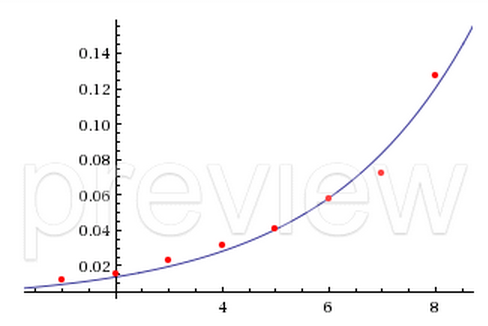
\includegraphics[width=0.5\textwidth]{bruteforceTimes.png}}
\caption{\emph{Runtime plot}: fits an exponetial curve: $0.00656518 e^{(0.363729
x)} $\cite{WolfA}}
\end{figure}
\end{center}
\FloatBarrier
This leads me to estimate that in one hour I can break:
\begin{equation*}
0.00656518e^(0.363729 x) = 3600\\
x = 36\\
2^{36} = 68719476736bit
\end{equation*}
Extending this to a year we get:
\begin{equation*}
0.00656518 e^(0.363729 x) = 30758400\\
x = 61\\
2^{61} = 2.305843\cdot10^{18}
\end{equation*}
Using a botnet of a milion I would be able to manage $2^{61}\cdot 1000000 =
2.305843\cdot10^{24}$ bits. over a year.
